\documentclass[12pt]{article}
%\usepackage{algpseudocode} 
%\usepackage{algo}
\usepackage{fullpage,url,amssymb,epsfig,color,xspace,tikz,amsmath}
\usetikzlibrary{shapes,positioning,calc,chains}
\usepackage[pdftitle={CS 240 Assignment 3},%
pdfsubject={University of Waterloo, CS 240, Fall 2021},%
pdfauthor={MP}]{hyperref}
\RequirePackage{pstricks,pst-node,pst-tree} % draw trees, requires using xetex
\newlength{\nodeLength}
\newcommand{\Node}{A}
\newcommand{\setnode}[1]{
	\settowidth{\nodeLength}{#1}
	\renewcommand{\Node}[1]{
		\Tcircle[name=#1]{\makebox[\nodeLength]{##1}}
	}
}
\setnode{99}

% \snode{ID}{NUMBER} becomes \node{ID}[item]{\ensuremath{NUMBER}}
\newcommand{\snode}[2]{\node(#1)[item]{\ensuremath{#2}}}

% \nodelabel{SUBSCRIPT} becomes \node[label]{\ensuremath{S_SUBSCRIPT}}
\newcommand{\nodelabel}[1]{\node[label]{\ensuremath{S_#1}}}

\newcommand{\quesbox}[2]{\begin{center} \framebox[.5\textwidth]{%
			\raisebox{-5mm}[0mm][#1]{\begin{minipage}[t]{.45\textwidth}%
					{\normalsize\sf #2}{\phantom{ans}}\end{minipage}}} \end{center}}
\newcommand{\ceil}[1]{\left\lceil#1\right\rceil}
\newcommand{\floor}[1]{\left\lfloor#1\right\rfloor}
\renewcommand{\thesubsection}{Problem \arabic{subsection}}
\definecolor{typo}{rgb}{0.75,0,0}
\definecolor{care}{rgb}{0,0,0}
\begin{document}
	
	\begin{center}
		{\Large\bf Assignment 3 Problem 4}\\
		\vspace{3mm}
	\end{center}
	
	\definecolor{care}{rgb}{0,0,0}
	\def\question#1{\item[\bf #1.]}
	\def\part#1{\item[\bf #1)]}
	\newcommand{\pc}[1]{\mbox{\textbf{#1}}} % pseudocode
	
	
	
	%%%%%%%%%%%%%%%%%%%%%%%%%%%%%%%%%%%%%%%%%%%%%%%%%%%%%%%%%%%%%
	%%% Problem 4
	
	\begin{enumerate}
		\part{a} Practice (not worth any marks): Starting with an empty skip list, insert the following keys in order: 22 31 77 7 21 42 using the following flip sequence:
		
		\begin{center}
			HHTHTHHHTHHTHTHT
		\end{center}
		
		You should obtain the skip list given in the next part.
		
		\part{b} Given the following skip list:
		
		\begin{center}
			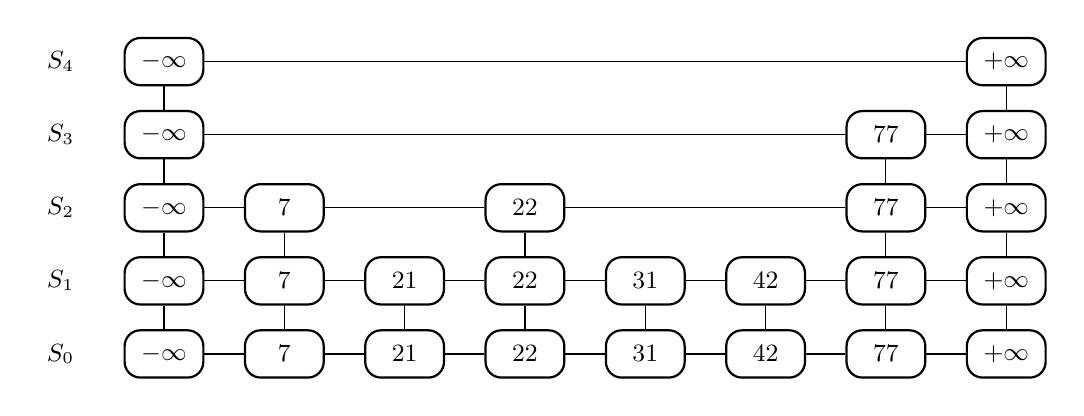
\begin{tikzpicture}[
				start chain,
				every node/.style={font=\small},
				item/.style={rectangle,minimum height=6mm,minimum width=10mm,
					rounded corners=2mm,thick,draw=black},
				label/.style={rectangle,minimum size=6mm}
				]
				
				% The nodes of the skip list are drawn in a matrix
				% \\ delimits the rows while & delimits the columns
				\matrix[row sep=3mm, column sep=5mm]{
					% Row 4: -infty ... +infty
					\nodelabel{4}; & \snode{4a}{-\infty}; & & & & & & & \snode{4n}{+\infty};\\
					
					% Row 3: -infty ... +infty
					\nodelabel{3}; & \snode{3a}{-\infty}; & & & & & & \snode{3l}{77}; & \snode{3n}{+\infty};\\
					
					% Row 2: -infty ...  ... +infty
					\nodelabel{2}; & \snode{2a}{-\infty}; & \snode{2c}{7}; & & \snode{2f}{22}; 
					& & & \snode{2l}{77}; & \snode{2n}{+\infty};\\
					
					% Row 1: -infty ...  ... +infty
					\nodelabel{1}; & \snode{1a}{-\infty}; & \snode{1c}{7}; & \snode{1e}{21}; & \snode{1f}{22}; 
					& \snode{1h}{31}; & \snode{1j}{42}; & \snode{1l}{77}; & \snode{1n}{+\infty};\\
					
					% Row 0: -infty 7 21 22 31 42 77 +infty
					\nodelabel{0}; & \snode{0a}{-\infty}; & \snode{0c}{7};  & \snode{0e}{21}; & \snode{0f}{22}; 
					& \snode{0h}{31};  & \snode{0j}{42};  & \snode{0l}{77};  & \snode{0n}{+\infty};\\
				};
				
				% Start chaining the nodes together
				{
					% Horizontal chains
					% Specify a starting node (by ID), and join to other nodes (by going "through" them in an unbroken line)
					% Eg row 2: Start at 2a, join 2e, join 2h, join 2i
					[start chain] \chainin(0a); \chainin(0c) [join]; \chainin(0e) [join]; \chainin(0f) [join]; \chainin(0h) [join];
					\chainin(0j) [join]; \chainin(0l) [join]; \chainin(0n) [join];
					[start chain] \chainin(1a); \chainin(1c) [join]; \chainin(1e) [join]; \chainin(1f) [join]; \chainin(1h) [join];
					\chainin(1j) [join]; \chainin(1l) [join]; \chainin(1n) [join];       
					[start chain] \chainin(2a); \chainin(2c) [join]; \chainin(2f) [join]; \chainin(2l) [join]; \chainin(2n) [join];
					[start chain] \chainin(3a); \chainin(3l) [join]; \chainin(3n) [join];
					[start chain] \chainin(4a); \chainin(4n) [join];
				}
				{
					% Vertical chains
					% Need to be separate chains from the horizontal ones
					[start chain] \chainin(0a); \chainin(1a) [join]; \chainin(2a) [join]; \chainin(3a) [join]; \chainin(4a) [join]; 
					[start chain] \chainin(0c); \chainin(1c) [join]; \chainin(2c) [join];
					[start chain] \chainin(0e); \chainin(1e) [join]; 
					[start chain] \chainin(0f); \chainin(1f) [join]; \chainin(2f) [join];
					[start chain] \chainin(0h); \chainin(1h) [join]; 
					[start chain] \chainin(0j); \chainin(1j) [join]; 
					[start chain] \chainin(0l); \chainin(1l) [join]; \chainin(2l) [join]; \chainin(3l) [join];
					[start chain] \chainin(0n); \chainin(1n) [join]; \chainin(2n) [join]; \chainin(3n) [join]; \chainin(4n) [join]; 
					
				}
			\end{tikzpicture}
		\end{center}
		
		
		Show the skip list that is created by inserting the keys: 37, 66, 13, 4, 27, 99 \\
		into the given skip list.  You must use the following coin flip sequence:
		\[
		HHHHTTHTHTHHTHTTHHHHHTHHTT
		\]
		Note that each coin flip in the sequence will only be used once, in order
		and there may be some unused coin flips.
		
		\begin{figure}[tbhp]
			\begin{center}
				\includegraphics[width=0.8\textwidth]{17.png}
			\end{center}
			\label{figcaption}
		\end{figure}
		
		After inserting all keys, determine the exact number of comparisons (between 2 keys) required to search for the keys inserted in this part (that is, indicate what the search cost would be for 37, and then the search cost for 66, and so on).
		
		For example, a search for 18 in the given skip list above, requires 6 comparisons.
		
		\begin{center}
			\begin{tabular}{|c||c|c|c|c|c|c|} \hline
				Key &  37 &  66 &  13 &  4 & 27 & 99 \\ \hline
				Comparisons & 10  & 8  & 7  & 6  & 8 & 8 \\ \hline
			\end{tabular}
		\end{center}
		
		For the remaining parts, assume that the probability of adding a level to a tower is $p$ ($0 < p < 1)$, as opposed to $\frac{1}{2}$.
		
		\part{c} Explain why the probability that a key in the skip list has height at least $i$ is $p^i$.
		
		Since the probability of adding a level to a tower is $p$, therefore, when we need a key that appears in the level i, the probability is $\underbrace{p \times p \times ... \times p}_{\text{i }p's} = p^i$, which also means that the probability of this key has height at least $i$ should be $p^i$ (since it appears in level i)
		
		\part{d} Show that the expected number of extra nodes (i.e., the total number of nodes in skip list not including the nodes in $S_0$) is $O(n)$. 
		Therefore, the space requirements for this skip list are linear in the number of keys being stored.
		
		Let $|S_i|$ be the number of keys in list $S_i$\\
		Let $X_k$ be the height of tower of key k, and $P(X_k\geq i)=p^i$\\
		Let $l_{i,k} = 0$ if $X_k < i$ and $l_{i,k} = 1$ if $X_k \geq i$\\
		$|S_i|=\sum_{\text{key k}} (l_{i,k})$\\
		$E(|S_i|)=E(\sum_{\text{key k}} (l_{i,k}))=\sum_{\text{key k}} E(l_{i,k}) = \sum_{\text{key k}} P(l_{i,k} = 1)=\sum_{\text{key k}} P(X_k\geq i)=np^i$\\
		Then, expected space for extra nodes should be $E(\sum_{i\geq 1}|S_i|) = \sum_{i\geq 1} np^i = \frac{np}{1-p} = \frac{p}{1-p} \times n \in O(n)$
		
	\end{enumerate}
	
\end{document}